\documentclass[]{article}
\usepackage{lmodern}
\usepackage{amssymb,amsmath}
\usepackage{ifxetex,ifluatex}
\usepackage{fixltx2e} % provides \textsubscript
\ifnum 0\ifxetex 1\fi\ifluatex 1\fi=0 % if pdftex
  \usepackage[T1]{fontenc}
  \usepackage[utf8]{inputenc}
\else % if luatex or xelatex
  \ifxetex
    \usepackage{mathspec}
  \else
    \usepackage{fontspec}
  \fi
  \defaultfontfeatures{Ligatures=TeX,Scale=MatchLowercase}
\fi
% use upquote if available, for straight quotes in verbatim environments
\IfFileExists{upquote.sty}{\usepackage{upquote}}{}
% use microtype if available
\IfFileExists{microtype.sty}{%
\usepackage{microtype}
\UseMicrotypeSet[protrusion]{basicmath} % disable protrusion for tt fonts
}{}
\usepackage[margin=1in]{geometry}
\usepackage{hyperref}
\hypersetup{unicode=true,
            pdftitle={Conditional Models},
            pdfauthor={Emorie D Beck},
            pdfborder={0 0 0},
            breaklinks=true}
\urlstyle{same}  % don't use monospace font for urls
\usepackage{color}
\usepackage{fancyvrb}
\newcommand{\VerbBar}{|}
\newcommand{\VERB}{\Verb[commandchars=\\\{\}]}
\DefineVerbatimEnvironment{Highlighting}{Verbatim}{commandchars=\\\{\}}
% Add ',fontsize=\small' for more characters per line
\usepackage{framed}
\definecolor{shadecolor}{RGB}{248,248,248}
\newenvironment{Shaded}{\begin{snugshade}}{\end{snugshade}}
\newcommand{\KeywordTok}[1]{\textcolor[rgb]{0.13,0.29,0.53}{\textbf{#1}}}
\newcommand{\DataTypeTok}[1]{\textcolor[rgb]{0.13,0.29,0.53}{#1}}
\newcommand{\DecValTok}[1]{\textcolor[rgb]{0.00,0.00,0.81}{#1}}
\newcommand{\BaseNTok}[1]{\textcolor[rgb]{0.00,0.00,0.81}{#1}}
\newcommand{\FloatTok}[1]{\textcolor[rgb]{0.00,0.00,0.81}{#1}}
\newcommand{\ConstantTok}[1]{\textcolor[rgb]{0.00,0.00,0.00}{#1}}
\newcommand{\CharTok}[1]{\textcolor[rgb]{0.31,0.60,0.02}{#1}}
\newcommand{\SpecialCharTok}[1]{\textcolor[rgb]{0.00,0.00,0.00}{#1}}
\newcommand{\StringTok}[1]{\textcolor[rgb]{0.31,0.60,0.02}{#1}}
\newcommand{\VerbatimStringTok}[1]{\textcolor[rgb]{0.31,0.60,0.02}{#1}}
\newcommand{\SpecialStringTok}[1]{\textcolor[rgb]{0.31,0.60,0.02}{#1}}
\newcommand{\ImportTok}[1]{#1}
\newcommand{\CommentTok}[1]{\textcolor[rgb]{0.56,0.35,0.01}{\textit{#1}}}
\newcommand{\DocumentationTok}[1]{\textcolor[rgb]{0.56,0.35,0.01}{\textbf{\textit{#1}}}}
\newcommand{\AnnotationTok}[1]{\textcolor[rgb]{0.56,0.35,0.01}{\textbf{\textit{#1}}}}
\newcommand{\CommentVarTok}[1]{\textcolor[rgb]{0.56,0.35,0.01}{\textbf{\textit{#1}}}}
\newcommand{\OtherTok}[1]{\textcolor[rgb]{0.56,0.35,0.01}{#1}}
\newcommand{\FunctionTok}[1]{\textcolor[rgb]{0.00,0.00,0.00}{#1}}
\newcommand{\VariableTok}[1]{\textcolor[rgb]{0.00,0.00,0.00}{#1}}
\newcommand{\ControlFlowTok}[1]{\textcolor[rgb]{0.13,0.29,0.53}{\textbf{#1}}}
\newcommand{\OperatorTok}[1]{\textcolor[rgb]{0.81,0.36,0.00}{\textbf{#1}}}
\newcommand{\BuiltInTok}[1]{#1}
\newcommand{\ExtensionTok}[1]{#1}
\newcommand{\PreprocessorTok}[1]{\textcolor[rgb]{0.56,0.35,0.01}{\textit{#1}}}
\newcommand{\AttributeTok}[1]{\textcolor[rgb]{0.77,0.63,0.00}{#1}}
\newcommand{\RegionMarkerTok}[1]{#1}
\newcommand{\InformationTok}[1]{\textcolor[rgb]{0.56,0.35,0.01}{\textbf{\textit{#1}}}}
\newcommand{\WarningTok}[1]{\textcolor[rgb]{0.56,0.35,0.01}{\textbf{\textit{#1}}}}
\newcommand{\AlertTok}[1]{\textcolor[rgb]{0.94,0.16,0.16}{#1}}
\newcommand{\ErrorTok}[1]{\textcolor[rgb]{0.64,0.00,0.00}{\textbf{#1}}}
\newcommand{\NormalTok}[1]{#1}
\usepackage{longtable,booktabs}
\usepackage{graphicx,grffile}
\makeatletter
\def\maxwidth{\ifdim\Gin@nat@width>\linewidth\linewidth\else\Gin@nat@width\fi}
\def\maxheight{\ifdim\Gin@nat@height>\textheight\textheight\else\Gin@nat@height\fi}
\makeatother
% Scale images if necessary, so that they will not overflow the page
% margins by default, and it is still possible to overwrite the defaults
% using explicit options in \includegraphics[width, height, ...]{}
\setkeys{Gin}{width=\maxwidth,height=\maxheight,keepaspectratio}
\IfFileExists{parskip.sty}{%
\usepackage{parskip}
}{% else
\setlength{\parindent}{0pt}
\setlength{\parskip}{6pt plus 2pt minus 1pt}
}
\setlength{\emergencystretch}{3em}  % prevent overfull lines
\providecommand{\tightlist}{%
  \setlength{\itemsep}{0pt}\setlength{\parskip}{0pt}}
\setcounter{secnumdepth}{0}
% Redefines (sub)paragraphs to behave more like sections
\ifx\paragraph\undefined\else
\let\oldparagraph\paragraph
\renewcommand{\paragraph}[1]{\oldparagraph{#1}\mbox{}}
\fi
\ifx\subparagraph\undefined\else
\let\oldsubparagraph\subparagraph
\renewcommand{\subparagraph}[1]{\oldsubparagraph{#1}\mbox{}}
\fi

%%% Use protect on footnotes to avoid problems with footnotes in titles
\let\rmarkdownfootnote\footnote%
\def\footnote{\protect\rmarkdownfootnote}

%%% Change title format to be more compact
\usepackage{titling}

% Create subtitle command for use in maketitle
\newcommand{\subtitle}[1]{
  \posttitle{
    \begin{center}\large#1\end{center}
    }
}

\setlength{\droptitle}{-2em}
  \title{Conditional Models}
  \pretitle{\vspace{\droptitle}\centering\huge}
  \posttitle{\par}
  \author{Emorie D Beck}
  \preauthor{\centering\large\emph}
  \postauthor{\par}
  \predate{\centering\large\emph}
  \postdate{\par}
  \date{9/7/2017}

% \usepackage[table]{xcolor}
\usepackage{array}
\usepackage{lscape}
\newcommand{\blandscape}{\begin{landscape}}
\newcommand{\elandscape}{\end{landscape}}
\usepackage{dcolumn}
\usepackage{bbm}
\usepackage{rotating, graphicx}
\usepackage{tabulary}
\usepackage{multirow}
\usepackage{algorithm}
\usepackage{booktabs}
\usepackage{colortbl}
\usepackage{longtable}
\usepackage{expex}
\usepackage{array}
\usepackage{multirow}
\usepackage{wrapfig}
\usepackage{float}
\usepackage{pdflscape}
\usepackage{tabu}
\usepackage{threeparttable}
\usepackage{booktabs}
\usepackage{longtable}
\usepackage{array}
\usepackage{multirow}
\usepackage[table]{xcolor}
\usepackage{wrapfig}
\usepackage{float}
\usepackage{colortbl}
\usepackage{pdflscape}
\usepackage{tabu}
\usepackage{threeparttable}

\begin{document}
\maketitle

{
\setcounter{tocdepth}{2}
\tableofcontents
}
\section{Workspace}\label{workspace}

\subsection{Packages}\label{packages}

\begin{Shaded}
\begin{Highlighting}[]
\KeywordTok{library}\NormalTok{(psych)}
\KeywordTok{library}\NormalTok{(sjPlot)}
\KeywordTok{library}\NormalTok{(broom)}
\KeywordTok{library}\NormalTok{(lme4)}
\KeywordTok{library}\NormalTok{(MuMIn)}
\KeywordTok{library}\NormalTok{(merTools)}
\KeywordTok{library}\NormalTok{(reghelper)}
\KeywordTok{library}\NormalTok{(stargazer)}
\KeywordTok{library}\NormalTok{(lsmeans)}
\KeywordTok{library}\NormalTok{(multcompView)}
\KeywordTok{library}\NormalTok{(plyr)}
\KeywordTok{library}\NormalTok{(tidyverse)}
\end{Highlighting}
\end{Shaded}

\section{Background}\label{background}

\subsection{Basic Syntex}\label{basic-syntex}

From last week:

\begin{itemize}
  \item \textbf{Level 1:} $Y_{ij} = \beta_{0j} + \varepsilon{ij}$
  \item \textbf{Level 2:} $\beta_{0j} = \gamma_{00} + U_{0j}$
\end{itemize}

\subsection{Sample Data}\label{sample-data}

The National Longitudinal Study of Youths 1979 Child and Young Adult
Sample (NLSYCYA) is a longitudinal study conducted by the National
Bureau of Labor Statistics. The sample includes the children of the
original 1979 sample. Here, we are going to use a subset of the more
than 11,000 variables available that include the following.

\begin{longtable}[]{@{}lll@{}}
\toprule
Item Name & Description & Time-Varying?\tabularnewline
\midrule
\endhead
PROC\_CID & Participant ID & No\tabularnewline
Dem\_DOB & Year of Date of Birth & No\tabularnewline
groups & Jail, Community Service, None & No\tabularnewline
DemPWeight & Weight Percentile at age 10 & No\tabularnewline
age & Age of participant & Yes\tabularnewline
Year & Year of Survey & Yes\tabularnewline
age0 & Age of participant (centered) & Yes\tabularnewline
SensSeek & Sensation-Seeking Composite & Yes\tabularnewline
CESD & CESD Depression Composite & Yes\tabularnewline
\bottomrule
\end{longtable}

\begin{Shaded}
\begin{Highlighting}[]
\NormalTok{data_path <-}\StringTok{ "https://github.com/longitudinal-data/1-descriptives-and-graphs-emoriebeck/raw/master/Conditional_Models"}
\KeywordTok{load}\NormalTok{(}\KeywordTok{url}\NormalTok{(}\KeywordTok{paste}\NormalTok{(data_path, }\StringTok{"sample.RData"}\NormalTok{, }\DataTypeTok{sep =} \StringTok{"/"}\NormalTok{)))}

\KeywordTok{head}\NormalTok{(sample_dat)}
\end{Highlighting}
\end{Shaded}

\begin{verbatim}
## # A tibble: 6 x 8
##   PROC_CID   age  year  age0   groups      CESD SensSeek DemPweight
##      <dbl> <dbl> <dbl> <dbl>   <fctr>     <dbl>    <dbl>      <dbl>
## 1     1601    16  2006     2 CommServ 0.4285714 3.666667  0.8159399
## 2     1601    18  2008     4 CommServ 2.0000000 3.000000  0.8159399
## 3     9102    16  2012     2     None 0.1818182 3.333333  0.6712397
## 4     9501    14  2000     0     Jail 0.5000000 3.000000  0.5477584
## 5     9501    18  2004     4     Jail 0.4285714 3.000000  0.5477584
## 6     9501    22  2008     8     Jail 0.4285714 3.000000  0.5477584
\end{verbatim}

\subsection{Simple Growth Curve Model}\label{simple-growth-curve-model}

\begin{itemize}
  \item \textbf{Level 1:} $Y_{ij} = \beta_{0j} + \beta_{1j}*time_{ij} + \varepsilon{ij}$
  \item \textbf{Level 2:} 
    \begin{itemize} 
      \item $\beta_{0j} = \gamma_{00} + U_{0j}$
      \item $\beta_{1j} = \gamma_{10} + U_{1j}$
    \end{itemize}
\end{itemize}

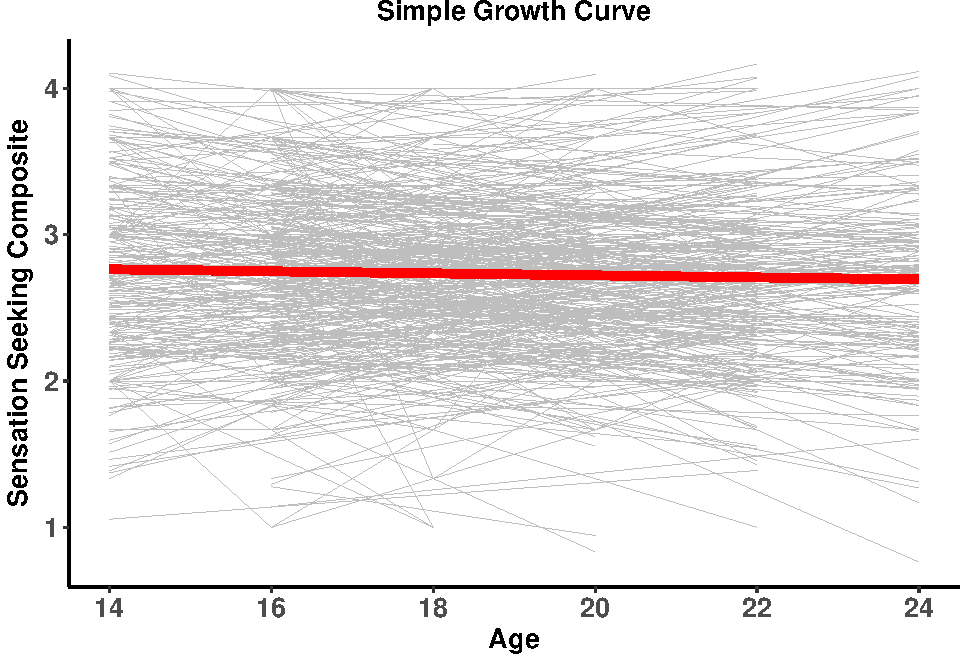
\includegraphics{Conditional_Models_doc_files/figure-latex/unnamed-chunk-3-1.pdf}

\subsection{In R}\label{in-r}

\small

\begin{Shaded}
\begin{Highlighting}[]
\NormalTok{mod0 <-}\StringTok{ }\KeywordTok{lmer}\NormalTok{(SensSeek }\OperatorTok{~}\StringTok{ }\NormalTok{age0 }\OperatorTok{+}\StringTok{ }\NormalTok{(}\DecValTok{1}\OperatorTok{|}\NormalTok{PROC_CID), }\DataTypeTok{data =}\NormalTok{ sample_dat)}
\end{Highlighting}
\end{Shaded}

\centering
\small

\begin{verbatim}
## Linear mixed model fit by REML ['lmerMod']
## Formula: SensSeek ~ age0 + (1 | PROC_CID)
##    Data: sample_dat
## 
## REML criterion at convergence: 3404.2
## 
## Scaled residuals: 
##     Min      1Q  Median      3Q     Max 
## -3.6782 -0.5396  0.0276  0.4739  3.2174 
## 
## Random effects:
##  Groups   Name        Variance Std.Dev.
##  PROC_CID (Intercept) 0.1349   0.3673  
##  Residual             0.2003   0.4475  
## Number of obs: 2084, groups:  PROC_CID, 924
## 
## Fixed effects:
##              Estimate Std. Error t value
## (Intercept)  2.765851   0.020067  137.83
## age0        -0.005879   0.003407   -1.73
## 
## Correlation of Fixed Effects:
##      (Intr)
## age0 -0.611
\end{verbatim}

\normalsize
\raggedright

\subsection{Conditional Models: Adding
Predictors}\label{conditional-models-adding-predictors}

Let's see if we can better predict participants' change in sensation
seeking over time by adding covariates.

\begin{longtable}[]{@{}lll@{}}
\toprule
Predictor & Continuous & Categorical\tabularnewline
\midrule
\endhead
Time Invariant & Weight for Age & Group\tabularnewline
Time Varying & CESD Scores & Depression\tabularnewline
\bottomrule
\end{longtable}

\section{Time Invariant Predictors}\label{time-invariant-predictors}

\subsection{Time Invariant Predictors:
Continuous}\label{time-invariant-predictors-continuous}

The basic equation, specifying a random intercept and slope:\\

\begin{itemize}
  \item \textbf{Level 1:} $Y_{ij} = \beta_{0j} + \beta_{1j}*time_{1j} + \varepsilon{ij}$
  \item \textbf{Level 2:} 
    \begin{itemize} 
      \item $\beta_{0j} = \gamma_{00} + \gamma_{01}*X_{2j} + U_{0j}$
      \item $\beta_{1j} = \gamma_{10} + \gamma_{11}*X_{2j} + U_{1j}$
    \end{itemize}
\end{itemize}

But we need to break this down to see that adding additional predictors
results in interaction terms:

\(Y_{ij} = \gamma_{00} + \gamma_{01}*X_{2j} + U_{0j} + (\gamma_{10} + \gamma_{11}*X_{2j} + U_{1j})*X_{1j} + \varepsilon{ij}\)
\(Y_{ij} = \gamma_{00} + \gamma_{01}*X_{2j} + \gamma_{10}*X_{1j} + \textcolor{red}{\gamma_{11}*X_{2j}*X_{1j}} + U_{0j} + U_{1j}*X_{1j} + \varepsilon{ij}\)

We can also fit this with intercepts depending on weight, but without
the change (slope) dependent on weight:\\
\(Y_{ij} = \gamma_{00} + \gamma_{01}*X_{2j} + U_{0j} + (\gamma_{10} + U_{1j})*X_{1j} + \varepsilon{ij}\)
\(Y_{ij} = \gamma_{00} + \gamma_{01}*X_{2j} + \gamma_{10}*X_{1j} + U_{0j} + U_{1j}*X_{1j} + \varepsilon{ij}\)

\subsubsection{Continuous Example - Weight for Age
Percentile}\label{continuous-example---weight-for-age-percentile}

\small

\begin{Shaded}
\begin{Highlighting}[]
\KeywordTok{describe}\NormalTok{(sample_dat}\OperatorTok{$}\NormalTok{DemPweight)}
\end{Highlighting}
\end{Shaded}

\begin{verbatim}
##    vars    n mean   sd median trimmed  mad   min  max range  skew kurtosis
## X1    1 2084 0.66 0.31   0.69    0.67 0.36 -0.06 1.62  1.68 -0.29    -0.56
##      se
## X1 0.01
\end{verbatim}

\normalsize

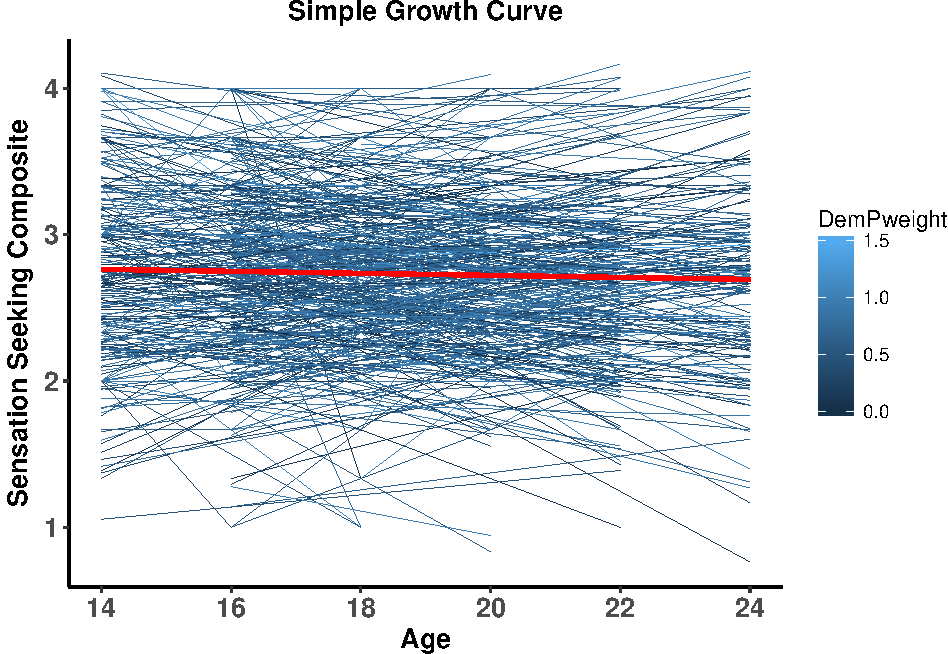
\includegraphics{Conditional_Models_doc_files/figure-latex/unnamed-chunk-7-1.pdf}

\small

\begin{Shaded}
\begin{Highlighting}[]
\CommentTok{# time invariant covariate with random intecept (with weight as covariate) }
\CommentTok{# and slope (without weight as a covariate)}
\NormalTok{mod1a <-}\StringTok{ }\KeywordTok{lmer}\NormalTok{(SensSeek }\OperatorTok{~}\StringTok{ }\NormalTok{age0 }\OperatorTok{+}\StringTok{ }\NormalTok{DemPweight }\OperatorTok{+}\StringTok{ }\NormalTok{(age0}\OperatorTok{|}\NormalTok{PROC_CID), }
              \DataTypeTok{data =}\NormalTok{ sample_dat)}

\KeywordTok{summary}\NormalTok{(mod1a)}

\CommentTok{# time invariant predictor with random slope and intercept}
\NormalTok{mod1b <-}\StringTok{ }\KeywordTok{lmer}\NormalTok{(SensSeek }\OperatorTok{~}\StringTok{ }\NormalTok{age0 }\OperatorTok{+}\StringTok{ }\NormalTok{DemPweight }\OperatorTok{+}\StringTok{ }\NormalTok{age0}\OperatorTok{*}\NormalTok{DemPweight }\OperatorTok{+}\StringTok{ }
\StringTok{                }\NormalTok{(age0}\OperatorTok{|}\NormalTok{PROC_CID), }\DataTypeTok{data =}\NormalTok{ sample_dat)}

\KeywordTok{summary}\NormalTok{(mod1b)}
\end{Highlighting}
\end{Shaded}

\normalsize

\subsection{Time Invariant Predictors:
Categorical}\label{time-invariant-predictors-categorical}

\subsubsection{Categorical Example - 2 level
group}\label{categorical-example---2-level-group}

Let's start with the basic syntax:

\begin{itemize}
  \item \textbf{Level 1:} $Y_{ij} = \beta_{0j} + \beta_{1j}*time_{1j} + \varepsilon{ij}$
  \item \textbf{Level 2:} 
    \begin{itemize} 
      \item $\beta_{0j} = \gamma_{00} + \gamma_{01}*X_{2j} + U_{0j}$
      \item $\beta_{1j} = \gamma_{10} + \gamma_{11}*X_{2j} + U_{1j}$
    \end{itemize}
\end{itemize}

Now let's swap that out for a 2 group sample from the present data:

\begin{itemize}
  \item \textbf{Level 1:} $Y_{ij} = \beta_{0j} + \beta_{1j}*age0_{ij} + \varepsilon{ij}$
  \item \textbf{Level 2:} 
    \begin{itemize} 
      \item $\beta_{0j} = \gamma_{00} + \gamma_{01}*groupsNone + U_{0j}$
      \item $\beta_{1j} = \gamma_{10} + \gamma_{11}*groupsNone + U_{1j}$
    \end{itemize}
\end{itemize}

\begin{longtable}[]{@{}ll@{}}
\toprule
Variable & D1\tabularnewline
\midrule
\endhead
Jail & 0\tabularnewline
None & 1\tabularnewline
\bottomrule
\end{longtable}

And plot it.\\
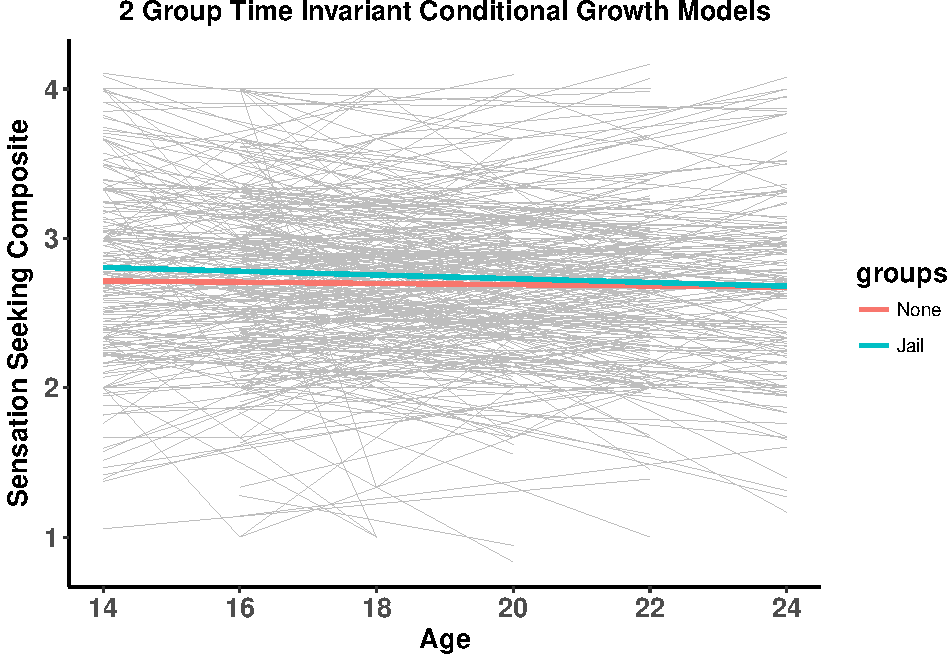
\includegraphics{Conditional_Models_doc_files/figure-latex/unnamed-chunk-9-1.pdf}

And model it:\\
\small

\begin{Shaded}
\begin{Highlighting}[]
\NormalTok{mod2g <-}\StringTok{ }\KeywordTok{lmer}\NormalTok{(SensSeek }\OperatorTok{~}\StringTok{ }\NormalTok{age0 }\OperatorTok{+}\StringTok{ }\NormalTok{groups }\OperatorTok{+}\StringTok{ }\NormalTok{age0}\OperatorTok{*}\NormalTok{groups }\OperatorTok{+}\StringTok{ }\NormalTok{(age0}\OperatorTok{|}\NormalTok{PROC_CID), }
              \DataTypeTok{data =}\NormalTok{ sample_dat }\OperatorTok\StringTok{ }\KeywordTok{filter}\NormalTok{(groups }\OperatorTok{!=}\StringTok{ "CommServ"}\NormalTok{))}
\KeywordTok{summary}\NormalTok{(mod2g)}
\end{Highlighting}
\end{Shaded}

\begin{verbatim}
## Linear mixed model fit by REML ['lmerMod']
## Formula: SensSeek ~ age0 + groups + age0 * groups + (age0 | PROC_CID)
##    Data: sample_dat %>% filter(groups != "CommServ")
## 
## REML criterion at convergence: 2607.6
## 
## Scaled residuals: 
##     Min      1Q  Median      3Q     Max 
## -3.2324 -0.4860  0.0463  0.4643  3.0578 
## 
## Random effects:
##  Groups   Name        Variance  Std.Dev. Corr 
##  PROC_CID (Intercept) 0.1613721 0.40171       
##           age0        0.0008963 0.02994  -0.31
##  Residual             0.1897644 0.43562       
## Number of obs: 1573, groups:  PROC_CID, 689
## 
## Fixed effects:
##                  Estimate Std. Error t value
## (Intercept)      2.717417   0.036423   74.61
## age0            -0.003998   0.006382   -0.63
## groupsJail       0.093497   0.048257    1.94
## age0:groupsJail -0.007432   0.008272   -0.90
## 
## Correlation of Fixed Effects:
##             (Intr) age0   grpsJl
## age0        -0.624              
## groupsJail  -0.755  0.471       
## age0:grpsJl  0.481 -0.772 -0.623
\end{verbatim}

\normalsize

\subsubsection{Categorical Example - 3 level
group}\label{categorical-example---3-level-group}

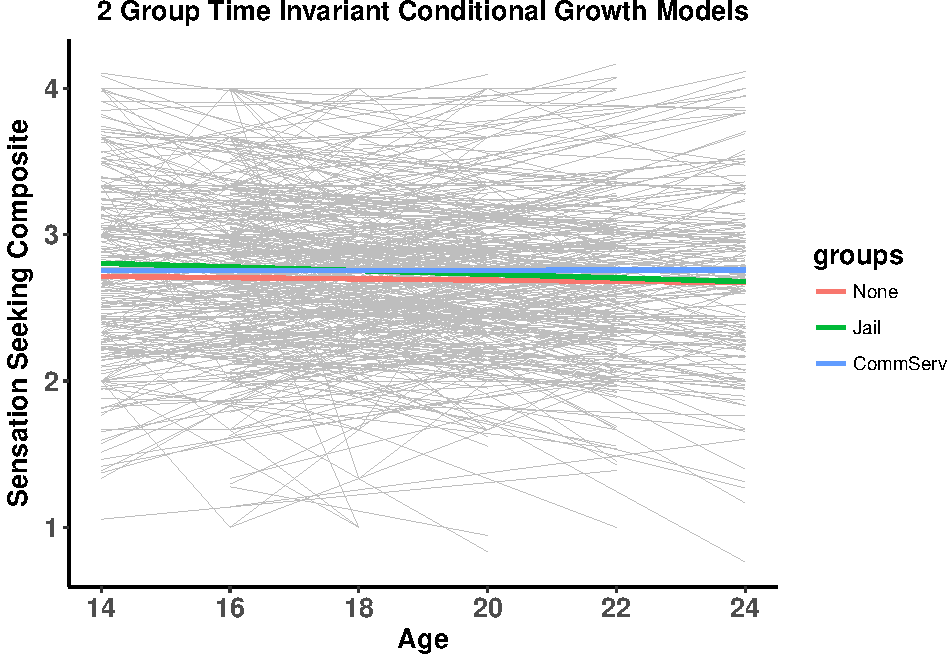
\includegraphics{Conditional_Models_doc_files/figure-latex/unnamed-chunk-11-1.pdf}

\begin{itemize}
  \item \textbf{Level 1:} $Y_{ij} = \beta_{0j} + \beta_{1j}*age0_{ij} + \varepsilon{ij}$
  \item \textbf{Level 2:} 
    \begin{itemize} 
      \item $\beta_{0j} = \gamma_{00} + \gamma_{01}*D1 + \gamma_{02}*D2 + U_{0j}$
      \item $\beta_{1j} = \gamma_{10} + \gamma_{11}*D1 + \gamma_{12}*D2 + U_{1j}$
    \end{itemize}
\end{itemize}

\begin{longtable}[]{@{}lll@{}}
\toprule
Variable & D1 & D2\tabularnewline
\midrule
\endhead
Jail & 0 & 0\tabularnewline
None & 1 & 0\tabularnewline
CommServ & 0 & 1\tabularnewline
\bottomrule
\end{longtable}

\small

\begin{Shaded}
\begin{Highlighting}[]
\NormalTok{mod3g <-}\StringTok{ }\KeywordTok{lmer}\NormalTok{(SensSeek }\OperatorTok{~}\StringTok{ }\NormalTok{age0 }\OperatorTok{+}\StringTok{ }\NormalTok{groups }\OperatorTok{+}\StringTok{ }\NormalTok{age0}\OperatorTok{*}\NormalTok{groups }\OperatorTok{+}\StringTok{ }
\StringTok{                }\NormalTok{(age0}\OperatorTok{|}\NormalTok{PROC_CID), }\DataTypeTok{data =}\NormalTok{ sample_dat)}
\KeywordTok{summary}\NormalTok{(mod3g)}
\end{Highlighting}
\end{Shaded}

\begin{verbatim}
## Linear mixed model fit by REML ['lmerMod']
## Formula: SensSeek ~ age0 + groups + age0 * groups + (age0 | PROC_CID)
##    Data: sample_dat
## 
## REML criterion at convergence: 3418.7
## 
## Scaled residuals: 
##     Min      1Q  Median      3Q     Max 
## -3.2994 -0.5006  0.0368  0.4533  3.0815 
## 
## Random effects:
##  Groups   Name        Variance  Std.Dev. Corr 
##  PROC_CID (Intercept) 0.1446194 0.38029       
##           age0        0.0008903 0.02984  -0.23
##  Residual             0.1888364 0.43455       
## Number of obs: 2084, groups:  PROC_CID, 924
## 
## Fixed effects:
##                      Estimate Std. Error t value
## (Intercept)          2.717703   0.035554   76.44
## age0                -0.004101   0.006376   -0.64
## groupsJail           0.092594   0.047097    1.97
## groupsCommServ       0.035192   0.053386    0.66
## age0:groupsJail     -0.007181   0.008265   -0.87
## age0:groupsCommServ  0.005939   0.009871    0.60
## 
## Correlation of Fixed Effects:
##             (Intr) age0   grpsJl grpsCS ag0:gJ
## age0        -0.619                            
## groupsJail  -0.755  0.467                     
## gropsCmmSrv -0.666  0.412  0.503              
## age0:grpsJl  0.478 -0.772 -0.618 -0.318       
## ag0:grpsCmS  0.400 -0.646 -0.302 -0.612  0.498
\end{verbatim}

\normalsize

\section{Side Notes: Practical
Applications}\label{side-notes-practical-applications}

\subsection{\texorpdfstring{Side Note: \texttt{lme4} helper
functions}{Side Note: lme4 helper functions}}\label{side-note-lme4-helper-functions}

\begin{Shaded}
\begin{Highlighting}[]
\KeywordTok{vcov}\NormalTok{(mod2g)}
\KeywordTok{VarCorr}\NormalTok{(mod2g)}
\KeywordTok{fixef}\NormalTok{(mod2g)}
\KeywordTok{head}\NormalTok{(}\KeywordTok{ranef}\NormalTok{(mod2g)[[}\DecValTok{1}\NormalTok{]])}
\KeywordTok{head}\NormalTok{(}\KeywordTok{coef}\NormalTok{(mod2g)[[}\DecValTok{1}\NormalTok{]])}
\KeywordTok{confint.merMod}\NormalTok{(mod2g, }\DataTypeTok{method =} \StringTok{"boot"}\NormalTok{)}
\NormalTok{reghelper}\OperatorTok{::}\KeywordTok{ICC}\NormalTok{(mod2g)}
\NormalTok{MuMIn}\OperatorTok{::}\KeywordTok{r.squaredGLMM}\NormalTok{(mod2g)}
\end{Highlighting}
\end{Shaded}

\small

\begin{Shaded}
\begin{Highlighting}[]
\KeywordTok{vcov}\NormalTok{(mod2g)}
\end{Highlighting}
\end{Shaded}

\begin{verbatim}
## 4 x 4 Matrix of class "dpoMatrix"
##                   (Intercept)          age0    groupsJail age0:groupsJail
## (Intercept)      0.0013266680 -1.449788e-04 -0.0013266680    1.449788e-04
## age0            -0.0001449788  4.072833e-05  0.0001449788   -4.072833e-05
## groupsJail      -0.0013266680  1.449788e-04  0.0023287011   -2.486054e-04
## age0:groupsJail  0.0001449788 -4.072833e-05 -0.0002486054    6.842322e-05
\end{verbatim}

\small

\begin{Shaded}
\begin{Highlighting}[]
\KeywordTok{VarCorr}\NormalTok{(mod2g)}
\end{Highlighting}
\end{Shaded}

\begin{verbatim}
##  Groups   Name        Std.Dev. Corr  
##  PROC_CID (Intercept) 0.401711       
##           age0        0.029938 -0.313
##  Residual             0.435620
\end{verbatim}

\small

\begin{Shaded}
\begin{Highlighting}[]
\KeywordTok{fixef}\NormalTok{(mod2g)}
\end{Highlighting}
\end{Shaded}

\begin{verbatim}
##     (Intercept)            age0      groupsJail age0:groupsJail 
##     2.717416961    -0.003997618     0.093496648    -0.007431764
\end{verbatim}

\small

\begin{Shaded}
\begin{Highlighting}[]
\KeywordTok{head}\NormalTok{(}\KeywordTok{ranef}\NormalTok{(mod2g)[[}\DecValTok{1}\NormalTok{]])}
\end{Highlighting}
\end{Shaded}

\begin{verbatim}
##       (Intercept)          age0
## 9102    0.2825889 -0.0036110312
## 9501    0.1582912  0.0013310875
## 9502    0.1542974 -0.0003923893
## 9503    0.1411350  0.0002529397
## 10001   0.1814453 -0.0008900323
## 12802   0.2999653 -0.0027624589
\end{verbatim}

\begin{Shaded}
\begin{Highlighting}[]
\KeywordTok{head}\NormalTok{(}\KeywordTok{coef}\NormalTok{(mod2g)[[}\DecValTok{1}\NormalTok{]])}
\end{Highlighting}
\end{Shaded}

\begin{verbatim}
##       (Intercept)         age0 groupsJail age0:groupsJail
## 9102     3.000006 -0.007608649 0.09349665    -0.007431764
## 9501     2.875708 -0.002666530 0.09349665    -0.007431764
## 9502     2.871714 -0.004390007 0.09349665    -0.007431764
## 9503     2.858552 -0.003744678 0.09349665    -0.007431764
## 10001    2.898862 -0.004887650 0.09349665    -0.007431764
## 12802    3.017382 -0.006760077 0.09349665    -0.007431764
\end{verbatim}

\small

\begin{Shaded}
\begin{Highlighting}[]
\KeywordTok{confint.merMod}\NormalTok{(mod2g, }\DataTypeTok{method =} \StringTok{"boot"}\NormalTok{, }\DataTypeTok{nsim =} \DecValTok{10}\NormalTok{)}
\end{Highlighting}
\end{Shaded}

\begin{verbatim}
##                       2.5 %       97.5 %
## .sig01           0.37825912  0.442446652
## .sig02          -0.59786608 -0.087752901
## .sig03           0.02074286  0.050678276
## .sigma           0.41349474  0.459740673
## (Intercept)      2.61954063  2.822716922
## age0            -0.01474274  0.004169720
## groupsJail       0.02965519  0.221246440
## age0:groupsJail -0.02043541  0.001165393
\end{verbatim}

All units of the random effects are in standard deviation units (which
means you need to square them to get the variance!!)\\

\begin{itemize}
  \item .sig01 = sd of random intercept = $\sqrt{\tau_{00}}$  
  \item .sig02 = correlation between slope and intercept = $\sqrt{\tau_{10}}$  
  \item .sig03 = sd of random slope = $\sqrt{\tau_{11}}$  
  \item .sigma = residual variance = $\hat{\sigma}$  
\end{itemize}

\small

\begin{Shaded}
\begin{Highlighting}[]
\NormalTok{reghelper}\OperatorTok{::}\KeywordTok{ICC}\NormalTok{(mod2g)}
\end{Highlighting}
\end{Shaded}

\begin{verbatim}
## [1] 0.4609468
\end{verbatim}

\begin{center}\rule{0.5\linewidth}{\linethickness}\end{center}

\small
\textbf{Conditional $R^2$:} How much variance fixed + random effects
explain\\
\textbf{Marginal $R^2$:} how much variance the fixed effects explain

\href{https://jonlefcheck.net/2013/03/13/r2-for-linear-mixed-effects-models/}{explained
here}

\begin{Shaded}
\begin{Highlighting}[]
\NormalTok{MuMIn}\OperatorTok{::}\KeywordTok{r.squaredGLMM}\NormalTok{(mod2g)}
\end{Highlighting}
\end{Shaded}

\begin{verbatim}
##         R2m         R2c 
## 0.005234242 0.452019164
\end{verbatim}

\normalsize

\subsection{Side Note: Creating MLM
Tables}\label{side-note-creating-mlm-tables}

There are lots of helpful packages for this, including
\texttt{stargazer} and \texttt{sjPlot}, which are demonstrated below.\\
\small

\begin{Shaded}
\begin{Highlighting}[]
\NormalTok{stargazer}\OperatorTok{::}\KeywordTok{stargazer}\NormalTok{(mod2g)}
\NormalTok{sjPlot}\OperatorTok{::}\KeywordTok{sjt.lmer}\NormalTok{(mod2g)}
\end{Highlighting}
\end{Shaded}

\normalsize

The problem is that \texttt{stargazer()} doesn't include all the terms
we want, and \texttt{sjt.lmer()} only renders html. Embedded in the
\texttt{.Rmd} version of these slides is some code that should help you
to extract the terms you need and create a table using \texttt{dplyr}
and \texttt{tidyr} that you can render in \LaTeX using
\texttt{stargazer}.

But let's understand where those variables came from. To do so, we'll
use the \texttt{broom} package in R to grab the terms we need.

\begin{longtable}[]{@{}ll@{}}
\toprule
Description & Math Notation\tabularnewline
\midrule
\endhead
Fixed Effect Intercept & \(\gamma_{00}\)\tabularnewline
Fixed Effect Group Intercept & \(\gamma_{01}\)\tabularnewline
Fixed Effect Age Slope & \(\gamma_{10}\)\tabularnewline
Fixed Effect Group Slope & \(\gamma_{11}\)\tabularnewline
Individual Random Intercepts & \(U_{0j}\)\tabularnewline
Variance of Random Intercepts & \(\tau_{00}\)\tabularnewline
Random Age Slopes & \(U_{10}\)\tabularnewline
Variance of Random Age Slopes & \(\tau_{11}\)\tabularnewline
Correlation b/w Random Slopes and Intercepts &
\(\tau_{10}\)\tabularnewline
Residual Variance & \(\hat{\sigma}^2\)\tabularnewline
Intraclass Correlation & ICC\tabularnewline
Conditional \(R^2\) & \(R^2_c\)\tabularnewline
Marginal \(R^2\) & \(R^2_m\)\tabularnewline
\bottomrule
\end{longtable}

\begin{Shaded}
\begin{Highlighting}[]
\NormalTok{broom}\OperatorTok{::}\KeywordTok{tidy}\NormalTok{(mod2g)}
\NormalTok{broom}\OperatorTok{::}\KeywordTok{glance}\NormalTok{(mod2g)}
\end{Highlighting}
\end{Shaded}

\small

\begin{verbatim}
##                            term     estimate   std.error  statistic
## 1                   (Intercept)  2.717416961 0.036423454 74.6062393
## 2                          age0 -0.003997618 0.006381875 -0.6264017
## 3                    groupsJail  0.093496648 0.048256617  1.9374887
## 4               age0:groupsJail -0.007431764 0.008271833 -0.8984423
## 5       sd_(Intercept).PROC_CID  0.401711448          NA         NA
## 6              sd_age0.PROC_CID  0.029938129          NA         NA
## 7 cor_(Intercept).age0.PROC_CID -0.312526843          NA         NA
## 8       sd_Observation.Residual  0.435619527          NA         NA
##      group
## 1    fixed
## 2    fixed
## 3    fixed
## 4    fixed
## 5 PROC_CID
## 6 PROC_CID
## 7 PROC_CID
## 8 Residual
\end{verbatim}

\begin{verbatim}
##       sigma    logLik      AIC      BIC deviance df.residual
## 1 0.4356195 -1303.786 2623.571 2666.457 2579.802        1565
\end{verbatim}

Below is code that \emph{should} work for all models. Just run the
function and save it as an \texttt{R} object. You can use this with
\texttt{papaja} and the \texttt{apa\_table()} function pretty easily.
The trick is that if you are not using the papaja template, the proper
LaTeX packages may not be loaded. You can get around this by attaching a
.tex file calling the packages under ``in\_header: header.tex'' in your
YAML header. The YAML header of this .Rmd file contains the necessary
syntax and the header.tex file with the proper packages.

\begin{Shaded}
\begin{Highlighting}[]
\NormalTok{## here's some code to make a table. You shouldn't need to modify anything here }
\CommentTok{# unless you add additional random effects terms}
\NormalTok{## fixed effects first ##}
\NormalTok{table_fun <-}\StringTok{ }\ControlFlowTok{function}\NormalTok{(model)\{}
\NormalTok{    fixed <-}\StringTok{ }\NormalTok{broom}\OperatorTok{::}\KeywordTok{tidy}\NormalTok{(mod2g) }\OperatorTok\StringTok{ }\KeywordTok{filter}\NormalTok{(group }\OperatorTok{==}\StringTok{ "fixed"}\NormalTok{) }\OperatorTok
\StringTok{    }\KeywordTok{select}\NormalTok{(term, estimate) }
\NormalTok{  ## add random effects ##}
\NormalTok{  rand <-}\StringTok{ }\NormalTok{broom}\OperatorTok{::}\KeywordTok{tidy}\NormalTok{(mod2g) }\OperatorTok\StringTok{ }\KeywordTok{filter}\NormalTok{(group }\OperatorTok{!=}\StringTok{ "fixed"}\NormalTok{) }\OperatorTok
\StringTok{    }\KeywordTok{select}\NormalTok{(term, estimate)}
\NormalTok{  ## get confidence intervals ##}
\NormalTok{  CI <-}\StringTok{ }\KeywordTok{data.frame}\NormalTok{(}\KeywordTok{confint.merMod}\NormalTok{(mod2g, }\DataTypeTok{method =} \StringTok{"boot"}\NormalTok{, }\DataTypeTok{nsim =} \DecValTok{10}\NormalTok{)) }\OperatorTok
\StringTok{    }\KeywordTok{mutate}\NormalTok{(}\DataTypeTok{term =} \KeywordTok{rownames}\NormalTok{(.)) }\OperatorTok\StringTok{ }\KeywordTok{setNames}\NormalTok{(}\KeywordTok{c}\NormalTok{(}\StringTok{"lower"}\NormalTok{, }\StringTok{"upper"}\NormalTok{, }\StringTok{"term"}\NormalTok{))}
  
\NormalTok{  ## Get ICC & R2 values ##}
\NormalTok{  ICC <-}\StringTok{ }\NormalTok{reghelper}\OperatorTok{::}\KeywordTok{ICC}\NormalTok{(mod2g)}
\NormalTok{  R2 <-}\StringTok{ }\NormalTok{MuMIn}\OperatorTok{::}\KeywordTok{r.squaredGLMM}\NormalTok{(mod2g)}
  
\NormalTok{  ## format the fixed effects}
\NormalTok{  fixed <-}\StringTok{ }\NormalTok{fixed }\OperatorTok\StringTok{ }\KeywordTok{left_join}\NormalTok{(CI }\OperatorTok\StringTok{ }\KeywordTok{filter}\NormalTok{(}\OperatorTok{!}\KeywordTok{grepl}\NormalTok{(}\StringTok{".sig"}\NormalTok{, term))) }\OperatorTok
\StringTok{    }\KeywordTok{mutate}\NormalTok{(}\DataTypeTok{type =} \StringTok{"Fixed Parts"}\NormalTok{)}
  
\NormalTok{  rand <-}\StringTok{ }\NormalTok{rand }\OperatorTok
\StringTok{    }\KeywordTok{mutate}\NormalTok{(}\DataTypeTok{term =} \KeywordTok{mapvalues}\NormalTok{(term, }\KeywordTok{unique}\NormalTok{(term), }
            \KeywordTok{c}\NormalTok{(}\StringTok{"$}\CharTok{\textbackslash{}\textbackslash{}}\StringTok{tau\{00\}$"}\NormalTok{, }\StringTok{"$}\CharTok{\textbackslash{}\textbackslash{}}\StringTok{tau_\{11\}$"}\NormalTok{, }\StringTok{"$}\CharTok{\textbackslash{}\textbackslash{}}\StringTok{tau_\{10\}$"}\NormalTok{, }\StringTok{"$}\CharTok{\textbackslash{}\textbackslash{}}\StringTok{hat\{}\CharTok{\textbackslash{}\textbackslash{}}\StringTok{sigma^2\}$"}\NormalTok{)),}
           \DataTypeTok{estimate =}\NormalTok{ estimate}\OperatorTok{^}\DecValTok{2}\NormalTok{) }\OperatorTok
\StringTok{    }\KeywordTok{left_join}\NormalTok{(}
\NormalTok{      CI }\OperatorTok\StringTok{ }\KeywordTok{filter}\NormalTok{(}\KeywordTok{grepl}\NormalTok{(}\StringTok{".sig"}\NormalTok{, term)) }\OperatorTok
\StringTok{        }\KeywordTok{mutate}\NormalTok{(}\DataTypeTok{term =} \KeywordTok{mapvalues}\NormalTok{(term, }\KeywordTok{unique}\NormalTok{(term), }
            \KeywordTok{c}\NormalTok{(}\StringTok{"$}\CharTok{\textbackslash{}\textbackslash{}}\StringTok{tau\{00\}$"}\NormalTok{, }\StringTok{"$}\CharTok{\textbackslash{}\textbackslash{}}\StringTok{tau_\{10\}$"}\NormalTok{, }\StringTok{"$}\CharTok{\textbackslash{}\textbackslash{}}\StringTok{tau_\{11\}$"}\NormalTok{, }\StringTok{"$}\CharTok{\textbackslash{}\textbackslash{}}\StringTok{hat\{}\CharTok{\textbackslash{}\textbackslash{}}\StringTok{sigma^2\}$"}\NormalTok{)),}
            \DataTypeTok{lower =}\NormalTok{ lower}\OperatorTok{^}\DecValTok{2}\NormalTok{, }\DataTypeTok{upper =}\NormalTok{ upper}\OperatorTok{^}\DecValTok{2}\NormalTok{)) }\OperatorTok
\StringTok{    }\KeywordTok{mutate}\NormalTok{(}\DataTypeTok{type =} \StringTok{"Random Parts"}\NormalTok{)}
  
\NormalTok{  mod_terms <-}\StringTok{ }\KeywordTok{tribble}\NormalTok{(}
    \OperatorTok{~}\NormalTok{term, }\OperatorTok{~}\NormalTok{estimate, }\OperatorTok{~}\NormalTok{type,}
    \StringTok{"ICC"}\NormalTok{, ICC, }\StringTok{"Model Terms"}\NormalTok{,}
    \StringTok{"$R^2_m$"}\NormalTok{, R2[}\DecValTok{1}\NormalTok{], }\StringTok{"Model Terms"}\NormalTok{,}
    \StringTok{"$R^2_c$"}\NormalTok{, R2[}\DecValTok{2}\NormalTok{], }\StringTok{"Model Terms"}
\NormalTok{  )}
  
\NormalTok{  tab <-}\StringTok{ }\NormalTok{fixed }\OperatorTok
\StringTok{    }\KeywordTok{full_join}\NormalTok{(rand) }\OperatorTok
\StringTok{    }\KeywordTok{mutate}\NormalTok{(}\DataTypeTok{CI =} \KeywordTok{sprintf}\NormalTok{(}\StringTok{"(%.2f, %.2f)"}\NormalTok{, lower, upper)) }\OperatorTok
\StringTok{    }\KeywordTok{select}\NormalTok{(}\OperatorTok{-}\NormalTok{lower, }\OperatorTok{-}\NormalTok{upper) }\OperatorTok
\StringTok{    }\KeywordTok{full_join}\NormalTok{(mod_terms) }\OperatorTok
\StringTok{    }\KeywordTok{mutate}\NormalTok{(}\DataTypeTok{estimate =} \KeywordTok{sprintf}\NormalTok{(}\StringTok{"%.2f"}\NormalTok{, estimate)) }\OperatorTok
\StringTok{    }\KeywordTok{select}\NormalTok{(type, }\KeywordTok{everything}\NormalTok{())}
\NormalTok{\}}
\CommentTok{# you can use this with papaja and the apa_table function pretty easily}
\CommentTok{# the trick is that if you are not using the papaja template, the proper}
\CommentTok{# LaTeX packages may not be loaded. You can get around this by attaching}
\CommentTok{# a .tex file calling the packages under "in_header: header.tex" in your YAML}
\CommentTok{# header the YAML header of this .Rmd file contains the necessary syntax and }
\CommentTok{# the header.tex file with the proper packages}

\NormalTok{tab <-}\StringTok{ }\KeywordTok{table_fun}\NormalTok{(mod2g)}
\end{Highlighting}
\end{Shaded}

\subsubsection{\texorpdfstring{Basic:
\texttt{kable()}}{Basic: kable()}}\label{basic-kable}

\small

\begin{Shaded}
\begin{Highlighting}[]
\KeywordTok{options}\NormalTok{(}\DataTypeTok{knitr.kable.NA =} \StringTok{''}\NormalTok{)}
\NormalTok{knitr}\OperatorTok{::}\KeywordTok{kable}\NormalTok{(tab, }\DataTypeTok{caption =} \StringTok{"Ugly MLM Table Example"}\NormalTok{)}
\end{Highlighting}
\end{Shaded}

\begin{longtable}[]{@{}llll@{}}
\caption{Ugly MLM Table Example}\tabularnewline
\toprule
type & term & estimate & CI\tabularnewline
\midrule
\endfirsthead
\toprule
type & term & estimate & CI\tabularnewline
\midrule
\endhead
Fixed Parts & (Intercept) & 2.72 & (2.65, 2.74)\tabularnewline
Fixed Parts & age0 & -0.00 & (-0.01, 0.01)\tabularnewline
Fixed Parts & groupsJail & 0.09 & (0.04, 0.18)\tabularnewline
Fixed Parts & age0:groupsJail & -0.01 & (-0.03, -0.00)\tabularnewline
Random Parts & \(\tau{00}\) & 0.16 & (0.14, 0.19)\tabularnewline
Random Parts & \(\tau_{11}\) & 0.00 & (0.00, 0.00)\tabularnewline
Random Parts & \(\tau_{10}\) & 0.10 & (1.00, 0.00)\tabularnewline
Random Parts & \(\hat{\sigma^2}\) & 0.19 & (0.17, 0.20)\tabularnewline
Model Terms & ICC & 0.46 &\tabularnewline
Model Terms & \(R^2_m\) & 0.01 &\tabularnewline
Model Terms & \(R^2_c\) & 0.45 &\tabularnewline
\bottomrule
\end{longtable}

\subsubsection{\texorpdfstring{More Advanced: \texttt{kable()} +
\texttt{kableExtra}}{More Advanced: kable() + kableExtra}}\label{more-advanced-kable-kableextra}

\small

\begin{Shaded}
\begin{Highlighting}[]
\KeywordTok{library}\NormalTok{(kableExtra)}
\KeywordTok{options}\NormalTok{(}\DataTypeTok{knitr.kable.NA =} \StringTok{''}\NormalTok{)}
\NormalTok{knitr}\OperatorTok{::}\KeywordTok{kable}\NormalTok{(tab }\OperatorTok\StringTok{ }\CommentTok{#select(-type) %>%}
\StringTok{    }\KeywordTok{mutate}\NormalTok{(}\DataTypeTok{term =} \KeywordTok{gsub}\NormalTok{(}\StringTok{"[()]"}\NormalTok{, }\StringTok{""}\NormalTok{, term)),}
             \DataTypeTok{caption =} \StringTok{"Not Quite Right kableExtra MLM Table Example"}\NormalTok{, }
    \DataTypeTok{format =} \StringTok{"latex"}\NormalTok{, }
    \CommentTok{#longtable = T, }
    \DataTypeTok{booktabs =}\NormalTok{ T, }\DataTypeTok{escape =}\NormalTok{ F) }\OperatorTok
\StringTok{  }\CommentTok{# group_rows("Fixed", 1,4) %>% }
\StringTok{  }\CommentTok{# group_rows("Random", 5,9) %>%}
\StringTok{  }\CommentTok{# group_rows("Model", 9,11) %>%}
\StringTok{  }\KeywordTok{collapse_rows}\NormalTok{(}\DecValTok{1}\NormalTok{) }\OperatorTok
\StringTok{  }\CommentTok{#kable_styling(latex_options = c("striped","repeat_header"),full_width = F)}
\StringTok{  }\KeywordTok{add_header_above}\NormalTok{(}\KeywordTok{c}\NormalTok{(}\StringTok{" "}\NormalTok{, }\StringTok{" "}\NormalTok{, }\StringTok{"Model 1"}\NormalTok{ =}\StringTok{ }\DecValTok{2}\NormalTok{))}
\end{Highlighting}
\end{Shaded}

\begin{table}

\caption{\label{tab:unnamed-chunk-27}Not Quite Right kableExtra MLM Table Example}
\centering
\begin{tabular}[t]{llll}
\toprule
\multicolumn{1}{c}{ } & \multicolumn{1}{c}{ } & \multicolumn{2}{c}{Model 1} \\
\cmidrule(l{2pt}r{2pt}){3-4}
type & term & estimate & CI\\
\midrule
 & Intercept & 2.72 & (2.65, 2.74)\\
\cmidrule{2-4}
 & age0 & -0.00 & (-0.01, 0.01)\\
\cmidrule{2-4}
 & groupsJail & 0.09 & (0.04, 0.18)\\
\cmidrule{2-4}
\multirow{-4}{*}{\raggedright\arraybackslash Fixed Parts} & age0:groupsJail & -0.01 & (-0.03, -0.00)\\
\cmidrule{1-4}
 & $\tau{00}$ & 0.16 & (0.14, 0.19)\\
\cmidrule{2-4}
 & $\tau_{11}$ & 0.00 & (0.00, 0.00)\\
\cmidrule{2-4}
 & $\tau_{10}$ & 0.10 & (1.00, 0.00)\\
\cmidrule{2-4}
Random Parts & $\hat{\sigma^2}$ & 0.19 & (0.17, 0.20)\\
 & ICC & 0.46 & \\
\cmidrule{2-4}
Model Terms & $R^2_m$ & 0.01 & \\
Model Terms & $R^2_c$ & 0.45 & \\
\bottomrule
\end{tabular}
\end{table}

\subsubsection{\texorpdfstring{Alternative: \texttt{papaja} +
\texttt{apa\_table()}}{Alternative: papaja + apa\_table()}}\label{alternative-papaja-apa_table}

\small

\begin{Shaded}
\begin{Highlighting}[]
\NormalTok{papaja}\OperatorTok{::}\KeywordTok{apa_table}\NormalTok{(tab }\OperatorTok\StringTok{ }\KeywordTok{select}\NormalTok{(}\OperatorTok{-}\NormalTok{type),}\DataTypeTok{caption =} \StringTok{"papaja MLM Table Example"}\NormalTok{, }
    \DataTypeTok{na_string =} \StringTok{""}\NormalTok{, }\DataTypeTok{stub_indents =} \KeywordTok{list}\NormalTok{(}\DataTypeTok{Fixed =} \KeywordTok{c}\NormalTok{(}\DecValTok{1}\OperatorTok{:}\DecValTok{4}\NormalTok{), }\DataTypeTok{Random =} \KeywordTok{c}\NormalTok{(}\DecValTok{5}\OperatorTok{:}\DecValTok{11}\NormalTok{)))}
\end{Highlighting}
\end{Shaded}

\begin{table}[tbp]
\begin{center}
\begin{threeparttable}
\caption{\label{tab:unnamed-chunk-28}papaja MLM Table Example}
\begin{tabular}{lll}
\toprule
term & \multicolumn{1}{c}{estimate} & \multicolumn{1}{c}{CI}\\
\midrule
Fixed &  & \\
\ \ \ (Intercept) & 2.72 & (2.65, 2.74)\\
\ \ \ age0 & -0.00 & (-0.01, 0.01)\\
\ \ \ groupsJail & 0.09 & (0.04, 0.18)\\
\ \ \ age0:groupsJail & -0.01 & (-0.03, -0.00)\\
Random &  & \\
\ \ \ $\tau{00}$ & 0.16 & (0.14, 0.19)\\
\ \ \ $\tau_{11}$ & 0.00 & (0.00, 0.00)\\
\ \ \ $\tau_{10}$ & 0.10 & (1.00, 0.00)\\
\ \ \ $\hat{\sigma^2}$ & 0.19 & (0.17, 0.20)\\
\ \ \ ICC & 0.46 & \\
\ \ \ $R^2_m$ & 0.01 & \\
\ \ \ $R^2_c$ & 0.45 & \\
\bottomrule
\end{tabular}
\end{threeparttable}
\end{center}
\end{table}

\normalsize

\subsection{Side Note: Plotting}\label{side-note-plotting}

\subsubsection{\texorpdfstring{Lazy Method: \texttt{sjPlot} +
\texttt{sjt.int()}}{Lazy Method: sjPlot + sjt.int()}}\label{lazy-method-sjplot-sjt.int}

\paragraph{Categorical}\label{categorical}

\small

\begin{Shaded}
\begin{Highlighting}[]
\KeywordTok{sjp.int}\NormalTok{(mod2g, }\DataTypeTok{type =} \StringTok{"eff"}\NormalTok{, }\DataTypeTok{p.kr =}\NormalTok{ F, }\DataTypeTok{swap.pred =}\NormalTok{ T)}
\end{Highlighting}
\end{Shaded}

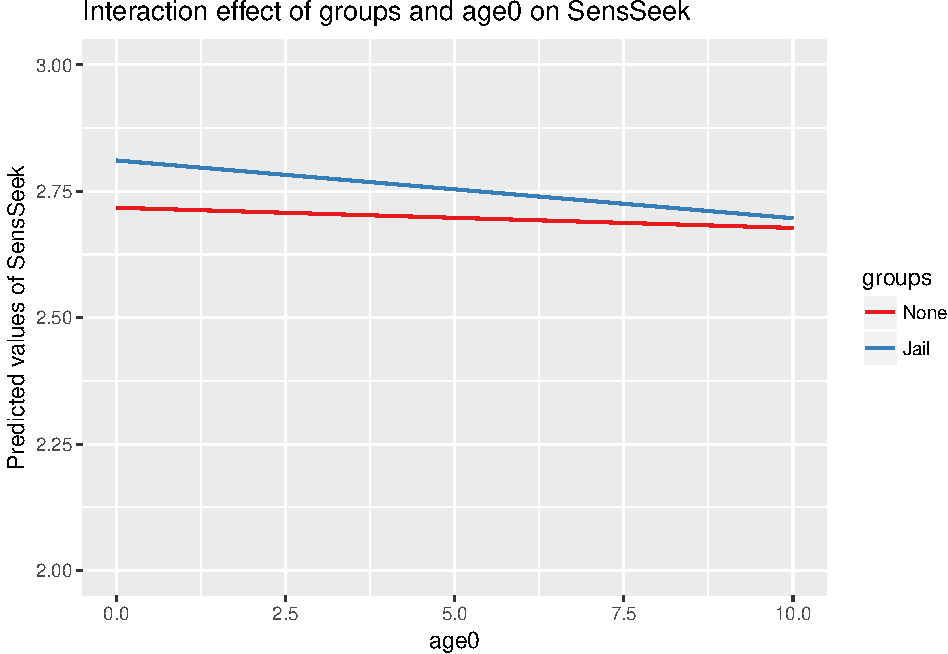
\includegraphics{Conditional_Models_doc_files/figure-latex/unnamed-chunk-29-1.pdf}

\paragraph{Continuous}\label{continuous}

\small

\begin{Shaded}
\begin{Highlighting}[]
\KeywordTok{sjp.int}\NormalTok{(mod1b, }\DataTypeTok{type =} \StringTok{"eff"}\NormalTok{, }\DataTypeTok{p.kr =}\NormalTok{ F, }\DataTypeTok{swap.pred =}\NormalTok{ T, }\DataTypeTok{mdrt.values =} \StringTok{"meansd"}\NormalTok{)}
\end{Highlighting}
\end{Shaded}

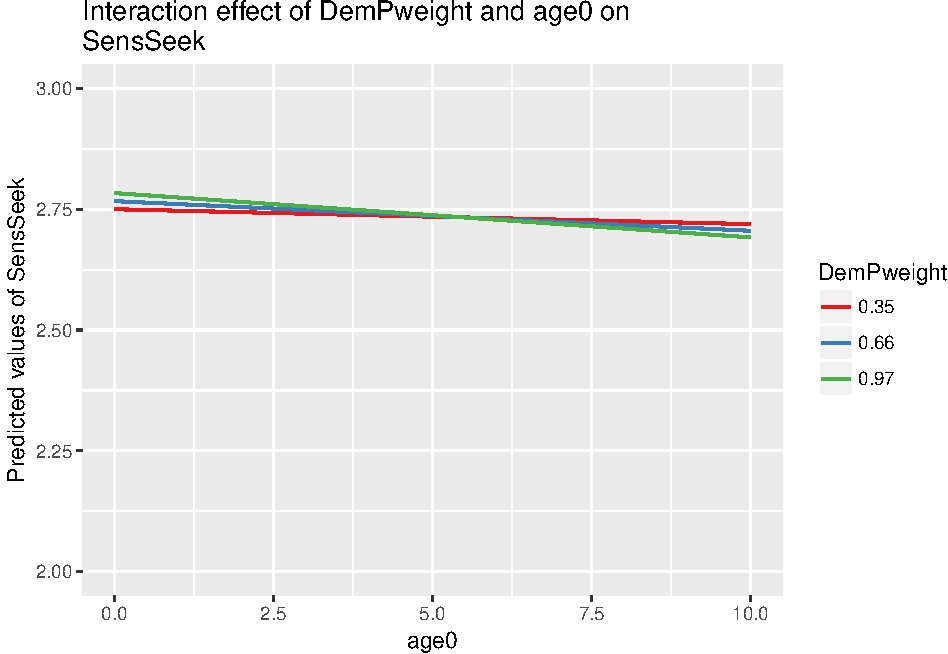
\includegraphics{Conditional_Models_doc_files/figure-latex/unnamed-chunk-30-1.pdf}

\subsubsection{\texorpdfstring{More advanced: \texttt{expand.grid()} +
\texttt{fixef()} +
\texttt{ggplot2()}}{More advanced: expand.grid() + fixef() + ggplot2()}}\label{more-advanced-expand.grid-fixef-ggplot2}

\paragraph{Categorical}\label{categorical-1}

\begin{Shaded}
\begin{Highlighting}[]
\CommentTok{# example for categorical}
\NormalTok{fixed.frame <-}\StringTok{ }
\StringTok{  }\KeywordTok{data.frame}\NormalTok{(}
    \KeywordTok{expand.grid}\NormalTok{(}
      \CommentTok{# here, you add values for your time variable and predictors}
      \DataTypeTok{age0 =} \KeywordTok{seq}\NormalTok{(}\DecValTok{0}\NormalTok{,}\DecValTok{10}\NormalTok{,}\DecValTok{2}\NormalTok{), }
      \DataTypeTok{groupsNone =} \KeywordTok{c}\NormalTok{(}\DecValTok{0}\NormalTok{,}\DecValTok{1}\NormalTok{))) }\OperatorTok
\StringTok{  }\CommentTok{# now take care of interactions and add an intercept}
\StringTok{  }\KeywordTok{mutate}\NormalTok{(}\StringTok{`}\DataTypeTok{age0:groupsNone}\StringTok{`}\NormalTok{ =}\StringTok{ }\NormalTok{age0}\OperatorTok{*}\NormalTok{groupsNone,}
         \DataTypeTok{Intercept =} \DecValTok{1}\NormalTok{) }\OperatorTok
\StringTok{  }\CommentTok{# reordering everything}
\StringTok{  }\KeywordTok{select}\NormalTok{(Intercept, }\KeywordTok{everything}\NormalTok{())}

\CommentTok{# multiplying to get values for model frame}
\NormalTok{fixed.frame}\OperatorTok{$}\NormalTok{value <-}\StringTok{ }\KeywordTok{as.vector}\NormalTok{(}\KeywordTok{as.matrix}\NormalTok{(fixed.frame) }\OperatorTok\StringTok{ }\KeywordTok{fixef}\NormalTok{(mod2g))}

\NormalTok{fixed.frame }\OperatorTok
\StringTok{  }\KeywordTok{mutate}\NormalTok{(}\DataTypeTok{groups =} \KeywordTok{factor}\NormalTok{(groupsNone, }\DataTypeTok{levels =} \KeywordTok{c}\NormalTok{(}\DecValTok{0}\NormalTok{,}\DecValTok{1}\NormalTok{), }\DataTypeTok{labels =} \KeywordTok{c}\NormalTok{(}\StringTok{"Jail"}\NormalTok{, }\StringTok{"None"}\NormalTok{)),}
         \DataTypeTok{age =}\NormalTok{ age0 }\OperatorTok{+}\StringTok{ }\DecValTok{14}\NormalTok{) }\OperatorTok
\StringTok{  }\KeywordTok{ggplot}\NormalTok{(}\KeywordTok{aes}\NormalTok{(}\DataTypeTok{x =}\NormalTok{ age, }\DataTypeTok{y =}\NormalTok{ value, }\DataTypeTok{color =}\NormalTok{ groups)) }\OperatorTok{+}
\StringTok{    }\KeywordTok{geom_line}\NormalTok{(}\DataTypeTok{size =} \DecValTok{2}\NormalTok{) }\OperatorTok{+}\StringTok{ }
\StringTok{    }\KeywordTok{labs}\NormalTok{(}\DataTypeTok{x =} \StringTok{"Age"}\NormalTok{, }\DataTypeTok{y =} \StringTok{"Sensation Seeking Composite"}\NormalTok{,}
         \DataTypeTok{title =} \StringTok{"2 Group Time Invariant Conditional Growth Models"}\NormalTok{) }\OperatorTok{+}
\StringTok{    }\KeywordTok{theme_classic}\NormalTok{() }\OperatorTok{+}
\StringTok{    }\KeywordTok{theme}\NormalTok{(}\DataTypeTok{axis.text =} \KeywordTok{element_text}\NormalTok{(}\DataTypeTok{face =} \StringTok{"bold"}\NormalTok{, }\DataTypeTok{size =} \KeywordTok{rel}\NormalTok{(}\FloatTok{1.2}\NormalTok{)),}
          \DataTypeTok{axis.title =} \KeywordTok{element_text}\NormalTok{(}\DataTypeTok{face =} \StringTok{"bold"}\NormalTok{, }\DataTypeTok{size =} \KeywordTok{rel}\NormalTok{(}\FloatTok{1.2}\NormalTok{)),}
          \DataTypeTok{legend.title =} \KeywordTok{element_text}\NormalTok{(}\DataTypeTok{face =} \StringTok{"bold"}\NormalTok{, }\DataTypeTok{size =} \KeywordTok{rel}\NormalTok{(}\FloatTok{1.2}\NormalTok{)),}
          \DataTypeTok{plot.title =} \KeywordTok{element_text}\NormalTok{(}\DataTypeTok{face =} \StringTok{"bold"}\NormalTok{, }\DataTypeTok{size =} \KeywordTok{rel}\NormalTok{(}\FloatTok{1.2}\NormalTok{), }\DataTypeTok{hjust =}\NormalTok{ .}\DecValTok{5}\NormalTok{))}
\end{Highlighting}
\end{Shaded}

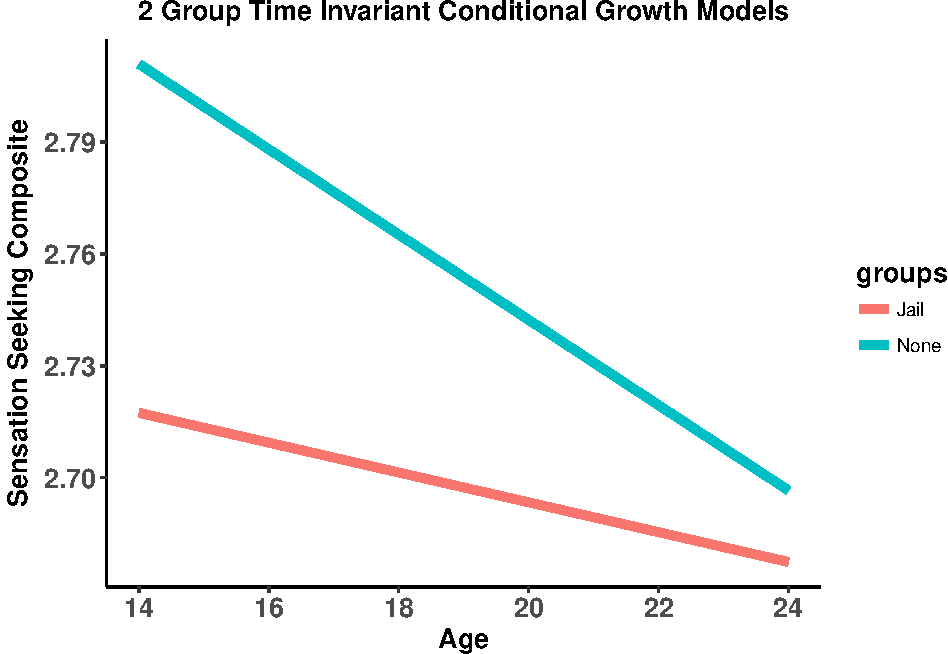
\includegraphics{Conditional_Models_doc_files/figure-latex/unnamed-chunk-31-1.pdf}

\paragraph{Continuous}\label{continuous-1}

\begin{Shaded}
\begin{Highlighting}[]
\CommentTok{# example for continuous}
\NormalTok{fixed.frame <-}\StringTok{ }\NormalTok{sample_dat }\OperatorTok
\StringTok{  }\KeywordTok{summarise}\NormalTok{(}\DataTypeTok{mean =} \KeywordTok{mean}\NormalTok{(DemPweight, }\DataTypeTok{na.rm =}\NormalTok{ T), }
            \DataTypeTok{sd =} \KeywordTok{sd}\NormalTok{(DemPweight, }\DataTypeTok{na.rm =}\NormalTok{ T))}

\NormalTok{fixed.frame <-}\StringTok{ }
\StringTok{  }\KeywordTok{data.frame}\NormalTok{(}
    \KeywordTok{expand.grid}\NormalTok{(}
      \CommentTok{# here, you add values for your time variable and predictors}
      \DataTypeTok{age0 =} \KeywordTok{seq}\NormalTok{(}\DecValTok{0}\NormalTok{,}\DecValTok{10}\NormalTok{,}\DecValTok{2}\NormalTok{), }
      \DataTypeTok{DemPweight =} \KeywordTok{c}\NormalTok{(fixed.frame}\OperatorTok{$}\NormalTok{mean}\OperatorTok{-}\NormalTok{fixed.frame}\OperatorTok{$}\NormalTok{sd,}
\NormalTok{                     fixed.frame}\OperatorTok{$}\NormalTok{mean,}
\NormalTok{                     fixed.frame}\OperatorTok{$}\NormalTok{mean}\OperatorTok{+}\NormalTok{fixed.frame}\OperatorTok{$}\NormalTok{sd))) }\OperatorTok
\StringTok{  }\CommentTok{# now take care of interactions and add an intercept}
\StringTok{  }\KeywordTok{mutate}\NormalTok{(}\StringTok{`}\DataTypeTok{age0:DemPweight}\StringTok{`}\NormalTok{ =}\StringTok{ }\NormalTok{age0}\OperatorTok{*}\NormalTok{DemPweight,}
         \DataTypeTok{Intercept =} \DecValTok{1}\NormalTok{) }\OperatorTok
\StringTok{  }\CommentTok{# reordering everything}
\StringTok{  }\KeywordTok{select}\NormalTok{(Intercept, }\KeywordTok{everything}\NormalTok{())}

\CommentTok{# multiplying to get values for model frame}
\NormalTok{fixed.frame}\OperatorTok{$}\NormalTok{value <-}\StringTok{ }\KeywordTok{as.vector}\NormalTok{(}\KeywordTok{as.matrix}\NormalTok{(fixed.frame) }\OperatorTok\StringTok{ }\KeywordTok{fixef}\NormalTok{(mod1b))}

\NormalTok{fixed.frame }\OperatorTok
\StringTok{  }\KeywordTok{mutate}\NormalTok{(}\DataTypeTok{Weight =} \KeywordTok{factor}\NormalTok{(DemPweight, }\DataTypeTok{levels =} \KeywordTok{unique}\NormalTok{(DemPweight), }\DataTypeTok{labels =} \KeywordTok{c}\NormalTok{(}\StringTok{"-1SD"}\NormalTok{, }\StringTok{"0SD"}\NormalTok{, }\StringTok{"1SD"}\NormalTok{)),}
         \DataTypeTok{age =}\NormalTok{ age0 }\OperatorTok{+}\StringTok{ }\DecValTok{14}\NormalTok{) }\OperatorTok
\StringTok{  }\KeywordTok{ggplot}\NormalTok{(}\KeywordTok{aes}\NormalTok{(}\DataTypeTok{x =}\NormalTok{ age, }\DataTypeTok{y =}\NormalTok{ value, }\DataTypeTok{color =}\NormalTok{ Weight)) }\OperatorTok{+}
\StringTok{    }\KeywordTok{geom_line}\NormalTok{(}\DataTypeTok{size =} \DecValTok{2}\NormalTok{) }\OperatorTok{+}\StringTok{ }
\StringTok{    }\KeywordTok{labs}\NormalTok{(}\DataTypeTok{x =} \StringTok{"Age"}\NormalTok{, }\DataTypeTok{y =} \StringTok{"Sensation Seeking Composite"}\NormalTok{,}
         \DataTypeTok{title =} \StringTok{"Continuous Invariant Conditional Growth Models"}\NormalTok{) }\OperatorTok{+}
\StringTok{    }\KeywordTok{theme_classic}\NormalTok{() }\OperatorTok{+}
\StringTok{    }\KeywordTok{theme}\NormalTok{(}\DataTypeTok{axis.text =} \KeywordTok{element_text}\NormalTok{(}\DataTypeTok{face =} \StringTok{"bold"}\NormalTok{, }\DataTypeTok{size =} \KeywordTok{rel}\NormalTok{(}\FloatTok{1.2}\NormalTok{)),}
          \DataTypeTok{axis.title =} \KeywordTok{element_text}\NormalTok{(}\DataTypeTok{face =} \StringTok{"bold"}\NormalTok{, }\DataTypeTok{size =} \KeywordTok{rel}\NormalTok{(}\FloatTok{1.2}\NormalTok{)),}
          \DataTypeTok{legend.title =} \KeywordTok{element_text}\NormalTok{(}\DataTypeTok{face =} \StringTok{"bold"}\NormalTok{, }\DataTypeTok{size =} \KeywordTok{rel}\NormalTok{(}\FloatTok{1.2}\NormalTok{)),}
          \DataTypeTok{plot.title =} \KeywordTok{element_text}\NormalTok{(}\DataTypeTok{face =} \StringTok{"bold"}\NormalTok{, }\DataTypeTok{size =} \KeywordTok{rel}\NormalTok{(}\FloatTok{1.2}\NormalTok{), }\DataTypeTok{hjust =}\NormalTok{ .}\DecValTok{5}\NormalTok{))}
\end{Highlighting}
\end{Shaded}

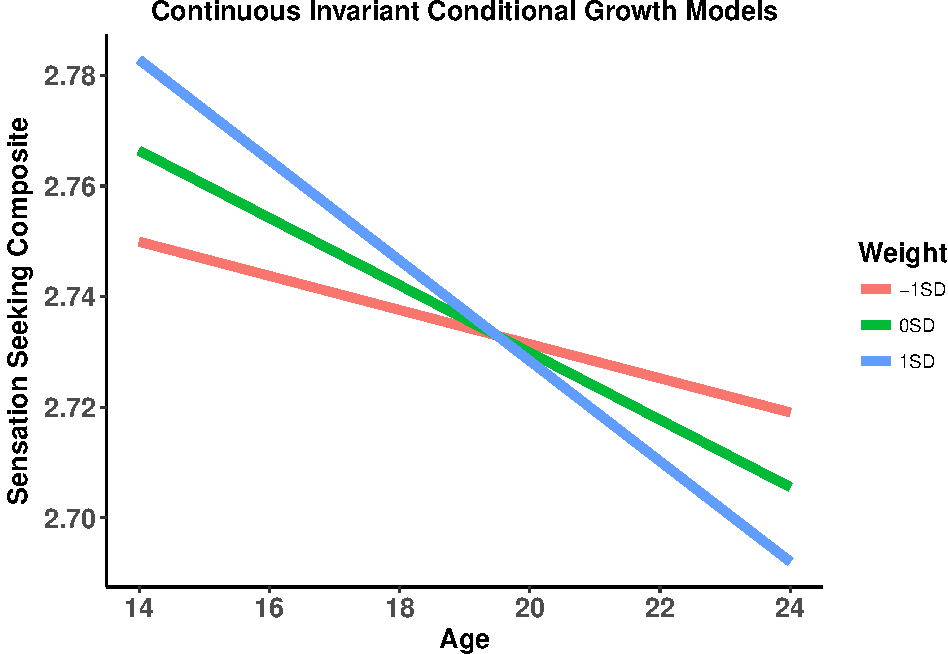
\includegraphics{Conditional_Models_doc_files/figure-latex/unnamed-chunk-32-1.pdf}

\normalsize  

\subsection{\texorpdfstring{Side Note: Comparisons with
\texttt{lsmeans}}{Side Note: Comparisons with lsmeans}}\label{side-note-comparisons-with-lsmeans}

The \texttt{lsmeans} package has a lot of useful functions. They are
listed below. Then I'll demonstrate them in turn.\\
\small

\begin{Shaded}
\begin{Highlighting}[]
\CommentTok{# create a reference grid}
\NormalTok{ref.grid2g <-}\StringTok{ }\KeywordTok{ref.grid}\NormalTok{(mod2g)}
\CommentTok{# create the lsmeans object}
\NormalTok{lsgroups   <-}\StringTok{ }\KeywordTok{lsmeans}\NormalTok{(ref.grid2g, }\StringTok{"groups"}\NormalTok{)}
\CommentTok{# compact letter display}
\KeywordTok{cld}\NormalTok{(lsgroups, }\DataTypeTok{alpha =}\NormalTok{ .}\DecValTok{10}\NormalTok{)}
\CommentTok{# plot}
\KeywordTok{plot}\NormalTok{(lsgroups)}
\CommentTok{# contrasts of the ref.grid object}
\KeywordTok{contrast}\NormalTok{(ref.grid2g, }\DataTypeTok{method =} \StringTok{"eff"}\NormalTok{)}
\CommentTok{# comparisons}
\NormalTok{groups.sum <-}\StringTok{ }\KeywordTok{summary}\NormalTok{(lsgroups, }\DataTypeTok{infer =} \KeywordTok{c}\NormalTok{(}\OtherTok{TRUE}\NormalTok{,}\OtherTok{TRUE}\NormalTok{), }
                      \DataTypeTok{level =}\NormalTok{ .}\DecValTok{90}\NormalTok{, }\DataTypeTok{adjust =} \StringTok{"bon"}\NormalTok{, }\DataTypeTok{by =} \StringTok{"groups"}\NormalTok{)}
\end{Highlighting}
\end{Shaded}

\begin{Shaded}
\begin{Highlighting}[]
\CommentTok{# create a reference grid}
\NormalTok{(ref.grid2g <-}\StringTok{ }\KeywordTok{ref.grid}\NormalTok{(mod2g))}
\end{Highlighting}
\end{Shaded}

\begin{verbatim}
## 'ref.grid' object with variables:
##     age0 = 3.9123
##     groups = None, Jail
\end{verbatim}

\begin{Shaded}
\begin{Highlighting}[]
\CommentTok{# create the lsmeans object}
\NormalTok{(lsgroups   <-}\StringTok{ }\KeywordTok{lsmeans}\NormalTok{(ref.grid2g, }\StringTok{"groups"}\NormalTok{))}
\end{Highlighting}
\end{Shaded}

\begin{verbatim}
##  groups   lsmean         SE     df lower.CL upper.CL
##  None   2.701777 0.02855972 701.42 2.645704 2.757850
##  Jail   2.766199 0.02480113 676.80 2.717505 2.814892
## 
## Degrees-of-freedom method: satterthwaite 
## Confidence level used: 0.95
\end{verbatim}

\begin{Shaded}
\begin{Highlighting}[]
\CommentTok{# compact letter display}
\KeywordTok{cld}\NormalTok{(lsgroups, }\DataTypeTok{alpha =}\NormalTok{ .}\DecValTok{10}\NormalTok{)}
\end{Highlighting}
\end{Shaded}

\begin{verbatim}
##  groups   lsmean         SE     df lower.CL upper.CL .group
##  None   2.701777 0.02855972 701.42 2.645704 2.757850  1    
##  Jail   2.766199 0.02480113 676.80 2.717505 2.814892   2   
## 
## Degrees-of-freedom method: satterthwaite 
## Confidence level used: 0.95 
## significance level used: alpha = 0.1
\end{verbatim}

\begin{Shaded}
\begin{Highlighting}[]
\CommentTok{# plot}
\KeywordTok{plot}\NormalTok{(lsgroups)}
\end{Highlighting}
\end{Shaded}

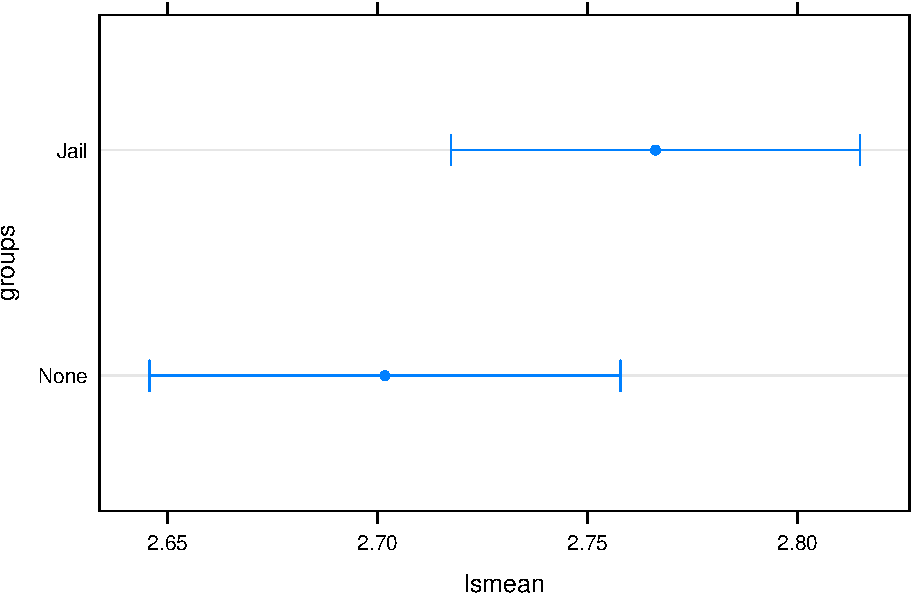
\includegraphics{Conditional_Models_doc_files/figure-latex/unnamed-chunk-37-1.pdf}

\begin{Shaded}
\begin{Highlighting}[]
\CommentTok{# contrasts of the ref.grid object}
\KeywordTok{contrast}\NormalTok{(ref.grid2g, }\DataTypeTok{method =} \StringTok{"eff"}\NormalTok{)}
\end{Highlighting}
\end{Shaded}

\begin{verbatim}
##  contrast                        estimate         SE     df t.ratio
##  3.91226954863318,None effect -0.03221079 0.01891265 690.74  -1.703
##  3.91226954863318,Jail effect  0.03221079 0.01891265 690.74   1.703
##  p.value
##   0.0890
##   0.0890
## 
## P value adjustment: fdr method for 2 tests
\end{verbatim}

\begin{Shaded}
\begin{Highlighting}[]
\CommentTok{# comparisons}
\NormalTok{(groups.sum <-}\StringTok{ }\KeywordTok{summary}\NormalTok{(lsgroups, }\DataTypeTok{infer =} \KeywordTok{c}\NormalTok{(}\OtherTok{TRUE}\NormalTok{,}\OtherTok{TRUE}\NormalTok{), }
          \DataTypeTok{level =}\NormalTok{ .}\DecValTok{90}\NormalTok{, }\DataTypeTok{adjust =} \StringTok{"bon"}\NormalTok{, }\DataTypeTok{by =} \StringTok{"groups"}\NormalTok{))}
\end{Highlighting}
\end{Shaded}

\begin{verbatim}
## groups = None:
##    lsmean         SE     df lower.CL upper.CL t.ratio p.value
##  2.701777 0.02855972 701.42 2.654739 2.748816  94.601  <.0001
## 
## groups = Jail:
##    lsmean         SE     df lower.CL upper.CL t.ratio p.value
##  2.766199 0.02480113 676.80 2.725351 2.807047 111.535  <.0001
## 
## Degrees-of-freedom method: satterthwaite 
## Confidence level used: 0.9
\end{verbatim}

\section{Time Varying Predictors}\label{time-varying-predictors}

\subsection{Time Varying Predictors:
Continuous}\label{time-varying-predictors-continuous}

Next, we'll add in a time-varying predictor. Maybe it's not that our
participants sensation seeking is moderated by early life experiences of
jail or court-ordered community service. Instead, their sensation
seeking is moderated by depression.\\
How does this look?

\begin{itemize}
  \item \textbf{Level 1:} $Y_{ij} = \beta_{0j} + \beta_{1j}*time + \beta_{2j}*CESD + \varepsilon{ij}$
  \item \textbf{Level 2:} 
    \begin{itemize} 
      \item $\beta_{0j} = \gamma_{00} + \gamma_{01} + U_{0j}$
      \item $\beta_{1j} = \gamma_{10} + U_{1j}$
      \item $\beta_{2j} = \gamma_{20}$
    \end{itemize}
\end{itemize}

\subsubsection{To Interaction or Not - That Is the
Question}\label{to-interaction-or-not---that-is-the-question}

\begin{itemize}
  \item \textbf{Level 1:} $Y_{ij} = \beta_{0j} + \beta_{1j}*age0 + \beta_{2j}*CESD + \varepsilon{ij}$
  \item \textbf{Level 2:} 
    \begin{itemize} 
      \item $\beta_{0j} = \gamma_{00} + \gamma_{01} + U_{0j}$
      \item $\beta_{1j} = \gamma_{10} + U_{1j}$
      \item $\beta_{2j} = \gamma_{20}$
    \end{itemize}
\end{itemize}

\[Y_{ij} =  \gamma_{00} + \gamma_{01} + U_{0j} + (\gamma_{10} + U_{1j})*age0 + \gamma_{20}*CESD\]

\subsubsection{Example: Does depression influence changes in sensation
seeking over
time?}\label{example-does-depression-influence-changes-in-sensation-seeking-over-time}

\small

\begin{Shaded}
\begin{Highlighting}[]
\NormalTok{modTV1 <-}\StringTok{ }\KeywordTok{lmer}\NormalTok{(SensSeek }\OperatorTok{~}\StringTok{ }\NormalTok{age0 }\OperatorTok{+}\StringTok{ }\NormalTok{CESD }\OperatorTok{+}\StringTok{ }\NormalTok{(age0}\OperatorTok{|}\NormalTok{PROC_CID), }\DataTypeTok{data =}\NormalTok{ sample_dat)}
\end{Highlighting}
\end{Shaded}

\small

\begin{Shaded}
\begin{Highlighting}[]
\KeywordTok{summary}\NormalTok{(modTV1)}
\end{Highlighting}
\end{Shaded}

\begin{verbatim}
## Linear mixed model fit by REML ['lmerMod']
## Formula: SensSeek ~ age0 + CESD + (age0 | PROC_CID)
##    Data: sample_dat
## 
## REML criterion at convergence: 3391.9
## 
## Scaled residuals: 
##     Min      1Q  Median      3Q     Max 
## -3.4390 -0.5035  0.0363  0.4423  3.1508 
## 
## Random effects:
##  Groups   Name        Variance  Std.Dev. Corr 
##  PROC_CID (Intercept) 0.1412389 0.37582       
##           age0        0.0008117 0.02849  -0.21
##  Residual             0.1892164 0.43499       
## Number of obs: 2084, groups:  PROC_CID, 924
## 
## Fixed effects:
##              Estimate Std. Error t value
## (Intercept)  2.710845   0.025121  107.91
## age0        -0.006475   0.003553   -1.82
## CESD         0.078617   0.021519    3.65
## 
## Correlation of Fixed Effects:
##      (Intr) age0  
## age0 -0.467       
## CESD -0.604 -0.036
\end{verbatim}

\normalsize

\begin{Shaded}
\begin{Highlighting}[]
\CommentTok{# example for continuous}
\CommentTok{# note MEANS ARE AT AGE0 = 0}
\NormalTok{fixed.frame <-}\StringTok{ }\NormalTok{sample_dat }\OperatorTok
\StringTok{  }\KeywordTok{filter}\NormalTok{(age0 }\OperatorTok{==}\StringTok{ }\DecValTok{0}\NormalTok{) }\OperatorTok
\StringTok{  }\KeywordTok{summarise}\NormalTok{(}\DataTypeTok{mean =} \KeywordTok{mean}\NormalTok{(CESD, }\DataTypeTok{na.rm =}\NormalTok{ T), }
            \DataTypeTok{sd =} \KeywordTok{sd}\NormalTok{(CESD, }\DataTypeTok{na.rm =}\NormalTok{ T))}

\NormalTok{fixed.frame <-}\StringTok{ }
\StringTok{  }\KeywordTok{data.frame}\NormalTok{(}
    \KeywordTok{expand.grid}\NormalTok{(}
      \CommentTok{# here, you add values for your time variable and predictors}
      \DataTypeTok{age0 =} \KeywordTok{seq}\NormalTok{(}\DecValTok{0}\NormalTok{,}\DecValTok{10}\NormalTok{,}\DecValTok{2}\NormalTok{), }
      \DataTypeTok{CESD =} \KeywordTok{c}\NormalTok{(fixed.frame}\OperatorTok{$}\NormalTok{mean}\OperatorTok{-}\NormalTok{fixed.frame}\OperatorTok{$}\NormalTok{sd,}
\NormalTok{                     fixed.frame}\OperatorTok{$}\NormalTok{mean,}
\NormalTok{                     fixed.frame}\OperatorTok{$}\NormalTok{mean}\OperatorTok{+}\NormalTok{fixed.frame}\OperatorTok{$}\NormalTok{sd))) }\OperatorTok
\StringTok{  }\CommentTok{# now take care of interactions and add an intercept}
\StringTok{  }\KeywordTok{mutate}\NormalTok{(}\DataTypeTok{Intercept =} \DecValTok{1}\NormalTok{) }\OperatorTok
\StringTok{  }\CommentTok{# reordering everything}
\StringTok{  }\KeywordTok{select}\NormalTok{(Intercept, }\KeywordTok{everything}\NormalTok{())}

\CommentTok{# multiplying to get values for model frame}
\NormalTok{fixed.frame}\OperatorTok{$}\NormalTok{value <-}\StringTok{ }\KeywordTok{as.matrix}\NormalTok{(fixed.frame) }\OperatorTok\StringTok{ }\KeywordTok{as.vector}\NormalTok{(}\KeywordTok{fixef}\NormalTok{(modTV1))}

\NormalTok{fixed.frame }\OperatorTok
\StringTok{  }\KeywordTok{mutate}\NormalTok{(}\DataTypeTok{CESD =} \KeywordTok{factor}\NormalTok{(CESD, }\DataTypeTok{levels =} \KeywordTok{unique}\NormalTok{(CESD), }\DataTypeTok{labels =} \KeywordTok{c}\NormalTok{(}\StringTok{"-1SD"}\NormalTok{, }\StringTok{"0SD"}\NormalTok{, }\StringTok{"1SD"}\NormalTok{)),}
         \DataTypeTok{age =}\NormalTok{ age0 }\OperatorTok{+}\StringTok{ }\DecValTok{14}\NormalTok{) }\OperatorTok
\StringTok{  }\KeywordTok{ggplot}\NormalTok{(}\KeywordTok{aes}\NormalTok{(}\DataTypeTok{x =}\NormalTok{ age, }\DataTypeTok{y =}\NormalTok{ value, }\DataTypeTok{color =}\NormalTok{ CESD)) }\OperatorTok{+}
\StringTok{    }\KeywordTok{geom_line}\NormalTok{(}\DataTypeTok{size =} \DecValTok{2}\NormalTok{) }\OperatorTok{+}\StringTok{ }
\StringTok{    }\KeywordTok{labs}\NormalTok{(}\DataTypeTok{x =} \StringTok{"Age"}\NormalTok{, }\DataTypeTok{y =} \StringTok{"Sensation Seeking Composite"}\NormalTok{,}
         \DataTypeTok{title =} \StringTok{"Continuous Time Varying Conditional Growth Models"}\NormalTok{) }\OperatorTok{+}
\StringTok{    }\KeywordTok{theme_classic}\NormalTok{() }\OperatorTok{+}
\StringTok{    }\KeywordTok{theme}\NormalTok{(}\DataTypeTok{axis.text =} \KeywordTok{element_text}\NormalTok{(}\DataTypeTok{face =} \StringTok{"bold"}\NormalTok{, }\DataTypeTok{size =} \KeywordTok{rel}\NormalTok{(}\FloatTok{1.2}\NormalTok{)),}
          \DataTypeTok{axis.title =} \KeywordTok{element_text}\NormalTok{(}\DataTypeTok{face =} \StringTok{"bold"}\NormalTok{, }\DataTypeTok{size =} \KeywordTok{rel}\NormalTok{(}\FloatTok{1.2}\NormalTok{)),}
          \DataTypeTok{legend.title =} \KeywordTok{element_text}\NormalTok{(}\DataTypeTok{face =} \StringTok{"bold"}\NormalTok{, }\DataTypeTok{size =} \KeywordTok{rel}\NormalTok{(}\FloatTok{1.2}\NormalTok{)),}
          \DataTypeTok{plot.title =} \KeywordTok{element_text}\NormalTok{(}\DataTypeTok{face =} \StringTok{"bold"}\NormalTok{, }\DataTypeTok{size =} \KeywordTok{rel}\NormalTok{(}\FloatTok{1.2}\NormalTok{), }\DataTypeTok{hjust =}\NormalTok{ .}\DecValTok{5}\NormalTok{))}
\end{Highlighting}
\end{Shaded}

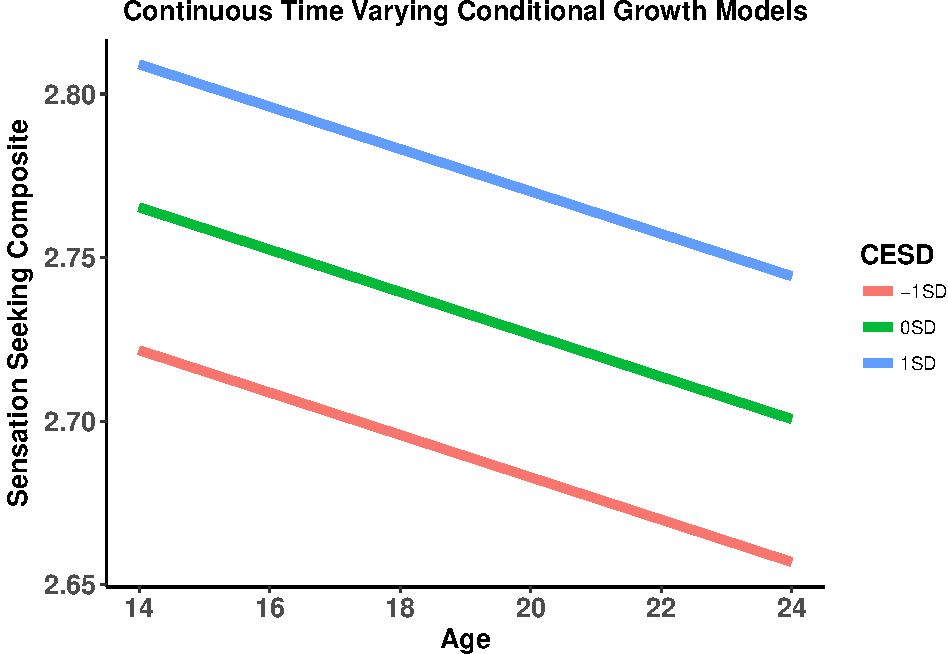
\includegraphics{Conditional_Models_doc_files/figure-latex/unnamed-chunk-42-1.pdf}

\subsection{Time Varying Predictors:
Categorical}\label{time-varying-predictors-categorical}

Next, we'll add in a time-varying predictor. Maybe it's not that our
participants sensation seeking is moderated by early life experiences of
jail or court-ordered community service. Instead, their sensation
seeking is moderated by depression.\\
How does this look?

\begin{itemize}
  \item \textbf{Level 1:} $Y_{ij} = \beta_{0j} + \beta_{1j}*time + \beta_{2j}*depressed + \varepsilon{ij}$
  \item \textbf{Level 2:} 
    \begin{itemize} 
      \item $\beta_{0j} = \gamma_{00} + \gamma_{01} + U_{0j}$
      \item $\beta_{1j} = \gamma_{10} + U_{1j}$
      \item $\beta_{2j} = \gamma_{20}$
    \end{itemize}
\end{itemize}

\small

\begin{Shaded}
\begin{Highlighting}[]
\CommentTok{# creating a dummy variable for time varying categorical depression}
\NormalTok{sample_dat <-}\StringTok{ }\NormalTok{sample_dat }\OperatorTok
\StringTok{  }\KeywordTok{mutate}\NormalTok{(}\DataTypeTok{depressed =} 
           \KeywordTok{factor}\NormalTok{(}\KeywordTok{ifelse}\NormalTok{(CESD }\OperatorTok{<=}\StringTok{ }\FloatTok{1.5}\NormalTok{, }\DecValTok{0}\NormalTok{, }\DecValTok{1}\NormalTok{), }\DataTypeTok{levels =} \KeywordTok{c}\NormalTok{(}\DecValTok{0}\NormalTok{,}\DecValTok{1}\NormalTok{), }
                  \DataTypeTok{labels =} \KeywordTok{c}\NormalTok{(}\StringTok{"Depressed"}\NormalTok{, }\StringTok{"Not Depressed"}\NormalTok{)))}
\NormalTok{modTV2 <-}\StringTok{ }\KeywordTok{lmer}\NormalTok{(SensSeek }\OperatorTok{~}\StringTok{ }\NormalTok{age0 }\OperatorTok{+}\StringTok{ }\NormalTok{depressed }\OperatorTok{+}\StringTok{ }\NormalTok{(age0}\OperatorTok{|}\NormalTok{PROC_CID), }
               \DataTypeTok{data =}\NormalTok{ sample_dat)}
\KeywordTok{summary}\NormalTok{(modTV2)}
\end{Highlighting}
\end{Shaded}

\begin{verbatim}
## Linear mixed model fit by REML ['lmerMod']
## Formula: SensSeek ~ age0 + depressed + (age0 | PROC_CID)
##    Data: sample_dat
## 
## REML criterion at convergence: 3401
## 
## Scaled residuals: 
##     Min      1Q  Median      3Q     Max 
## -3.3686 -0.5094  0.0363  0.4522  3.1406 
## 
## Random effects:
##  Groups   Name        Variance  Std.Dev. Corr 
##  PROC_CID (Intercept) 0.1427349 0.37780       
##           age0        0.0008415 0.02901  -0.21
##  Residual             0.1895332 0.43535       
## Number of obs: 2084, groups:  PROC_CID, 924
## 
## Fixed effects:
##                         Estimate Std. Error t value
## (Intercept)             2.760189   0.020388  135.38
## age0                   -0.006154   0.003564   -1.73
## depressedNot Depressed  0.068617   0.039992    1.72
## 
## Correlation of Fixed Effects:
##             (Intr) age0  
## age0        -0.599       
## dprssdNtDpr -0.174 -0.024
\end{verbatim}

\normalsize


\end{document}
